%\documentclass[draft]{beamer}%\documentclass[]{beamer}
\documentclass[]{beamer}%\documentclass[draft]{beamer}
\mode<presentation>
{
%  \usetheme{Boadilla}
  \usetheme{Frankfurt}
  \usecolortheme{crane}
}


\usepackage{graphicx}
\usepackage{hyperref}
%\usepackage[export]{adjustbox}

\title{JEE Choice filling Web Application and Seat-Allocation: A CS251 Report by Group 11.}
\author{
	Anmol Arora \\
   \texttt{Roll No. 130050027
    anmolarora59@gmail.com}\\
\and
Pranjal Khare \\
    \texttt{Roll No. 130050028 
    pranjalkhare7@gmail.com}\\
\and
Aman Goel \\
    \texttt{Roll No. 130050041 
    amangoelvsec@gmail.com}\\
}
\date{Oct 31, 2014}
\setbeamerfont{fig_font}{size=\small}
\setbeamercovered{invisible}
\usefonttheme[onlysmall]{structurebold}
% Delete this, if you do not want the table of contents to pop up at
% the beginning of each subsection:
% \AtBeginSubsection[]
% {
%   \begin{frame}<beamer>{Outline}
%     \tableofcontents[currentsection,currentsubsection]
%   \end{frame}
% }

% End Beamer stuff
\begin{document}

\begin{frame}
\titlepage
\end{frame}

\begin{frame}
	\frametitle{Overview} 
	\begin{columns}
	\column{0.5\textwidth}	
		\tableofcontents[] 
	\column{0.5\textwidth}
		\begin{figure}
		
\includegraphics[width=4cm ,height=2cm]{box2d.jpg}
		\end{figure}
	
	\end{columns}
\end{frame}


\section{Introduction}
\begin{frame}
	\frametitle{The Purpose of this Report}
	We created a web application that helps a candidate to fill his/her choices for JEE counselling. \pause 
	We also created a program in java that takes into account the preferences of students and the merit lists of the colleges \\
	in order to best allocate seats. \pause
	
	This report is made through beamer which is a very useful tool. It is much more powerful than other presentation softwares such as MS Power Point. \pause
	There are many predefined templates , which can be applied very easily, and make the presentation attractive and interactive.\pause
	
	
	
\end{frame}


\section{Body}

\subsection{Part 1: Pendulum}

\begin{frame}
\frametitle{Part 1: Pendulum}
\center
The Formula for the time period of a pendulum is: \cite{pendulum_time_period}\pause
\begin{equation}
	T = 2\pi \sqrt {\frac{l}{g}}
\end{equation}
\begin{flushleft}
\begin{itemize}
\pause
\item Here $ l $ is the length of thread from bob to pivot point and $ g $ is the acceleration due to gravity($ \approx 9.81 m/sec^2 $)\pause
\item $ g $ is the acceleration due to gravity.\\ \pause
\item $ v_x $ id the initial velocity of ball in x-direction (No acceleration in x-direction).\pause
\end{itemize}
\end{flushleft}
\begin{figure}
		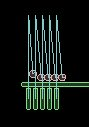
\includegraphics[width=2.5cm,height=2.5cm,keepaspectratio]{pendulum.jpg}
\end{figure}
\end{frame}

\subsection{Part 2: Flying Ball}

\begin{frame}
\frametitle{Part 2: Flying Ball}
\center
The equation of motion of a ball in free fall is: \cite{freeFall}\\
\begin{equation}
	s_y = u_y t + \frac{1}{2}gt^2
\end{equation}
\begin{equation}
	s_x = v_x t
\end{equation}
\begin{flushleft}
\begin{itemize}
\item $ s_y $ is the displacement in the y direction and $ s_x $ is the dispacement in x direction.\pause \\
\item $ g $ is the acceleration due to gravity.\pause \\
\item $ v_x $ id the initial velocity of ball in x-direction (No acceleration in x-direction).\pause
\end{itemize}
\end{flushleft}
\begin{figure}
		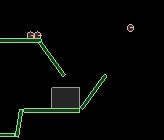
\includegraphics[width=2.5cm,height=2.5cm,keepaspectratio]{flyingball.jpg}
\end{figure}
\end{frame}


\subsection{Part 3: Collision}
\begin{frame}
	\frametitle{Part 3: Collision}
	\center
	Collision is dependent on the surfaces involved to a large extent. The principle equations involved are:\cite{Collision} \pause \\
	
	\begin{equation}
		m_1 v_{i1} + m_2 v_{i2} = m_1 v_{f1} + m_2 v_{f2}
	\end{equation}
	\pause
	\begin{equation}
		e = \frac{v_{f2} - v_{f1}}{v_{i2}-v_{i1}}
	\end{equation}	
	\pause
	\begin{columns}
	\column{0.7\textwidth}	
		\begin{itemize}
			\item e is a constant for two surfaces and is called  coefficient of restituion .It is dimensionless.\\\pause
			%\item $ m_1 $ and $ m_2 $ are the masses of bodies 1 and 2.\\
			\item $ v_{1i} $ ,$ v_{1f} $ , $ v_{2i} $ and $ v_{2f} $ are the velocities of body 1 and body 2 before and after the collision.\\\pause
		\end{itemize}
	\column{0.3\textwidth}
		\begin{figure}
			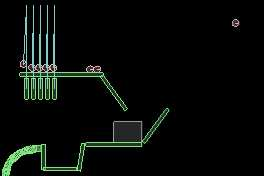
\includegraphics[width=2.5cm,height=2.5cm]{collision.jpg}
		\end{figure}
	\end{columns}
\end{frame}

\section{Conclusion}
\begin{frame}
	\frametitle{Conclusion}
	We did enjoy a lot, and learning Java and Django was a great experience in itself \pause \\
	We had chosen to drop the idea of Box2D and the 3 of us decided to rather do the \pause \\
	(Lab 10 + Lab 11) Pro Version project \pause \\
	We realised that Learning Python and Java would be of much more utility \pause \\
	It will be better to learn 2 highly popular programming languages \pause \\
	than just learning Box2D \pause \\
	Also, both of these languages are currently widely in use \pause \\
	So we decided that it was a better idea to learn python and java \pause \\
\end{frame}
\begin{frame}
	Another important reason was the beauty of the problem statement of Lab 10 and 11 \pause \\
	The problem statement wanted us to create a real time working \pause \\
	web application which was indeed fascinating \pause \\
	We had just learnt the Gale - Shapley algorithm in our Discrete Structures \pause \\
	course and a project which required an implementation of a recently learnt \pause \\
	algorithm sounded pretty cool to us \pause \\
	Java is a highly user friendly language to work with \pause \\
	It is fast, and is also highly efficient with a number of standard libraries that ease our task \pause \\
	Similarly, python is very easy to work with  \pause \\
	Django framework is a bit difficult to understand but once understood well,  \pause \\
	It can be used to make a wide variety of powerful web applications \pause \\
	All in all, we learnt a lot and we look forward to many other such projects in future \pause \\

\end{frame}


\section{References}
\begin{frame}
	\frametitle{References}
	\bibliographystyle{plain}
	\bibliography{simplebib}
\end{frame}


\end{document}


